\documentclass[11pt,fleqn]{article}
\usepackage{ee122,latexsym,epsf}
\usepackage{rotating}
\usepackage{amsmath,amssymb,enumerate,pgfplots}
\usepackage[ruled,vlined]{algorithm2e}
\lecture{1}
\def\title{HW \the\lecturenumber, Manohar Jois}
\begin{document}
\maketitle

% !TEX TS-program = pdflatex
% !TEX encoding = UTF-8 Unicode

% This is a simple template for a LaTeX document using the "article" class.
% See "book", "report", "letter" for other types of document.

%\documentclass[11pt]{article} % use larger type; default would be 10pt

%\usepackage[utf8]{inputenc} % set input encoding (not needed with XeLaTeX)

%%% Examples of Article customizations
% These packages are optional, depending whether you want the features they provide.
% See the LaTeX Companion or other references for full information.

%%% PAGE DIMENSIONS
%\usepackage{geometry} % to change the page dimensions
%\geometry{a4paper} % or letterpaper (US) or a5paper or....
% \geometry{margin=2in} % for example, change the margins to 2 inches all round
% \geometry{landscape} % set up the page for landscape
%   read geometry.pdf for detailed page layout information

%\usepackage{graphicx} % support the \includegraphics command and options

% \usepackage[parfill]{parskip} % Activate to begin paragraphs with an empty line rather than an indent

%%% PACKAGES
%\usepackage{amsmath, amsfonts}
%\usepackage{booktabs} % for much better looking tables
%\usepackage{array} % for better arrays (eg matrices) in maths
%\usepackage{paralist} % very flexible & customisable lists (eg. enumerate/itemize, etc.)
%\usepackage{verbatim} % adds environment for commenting out blocks of text & for better verbatim
%\usepackage{subfig} % make it possible to include more than one captioned figure/table in a single float
% These packages are all incorporated in the memoir class to one degree or another...

%%% HEADERS & FOOTERS
%\usepackage{fancyhdr} % This should be set AFTER setting up the page geometry
%\pagestyle{fancy} % options: empty , plain , fancy
%\renewcommand{\headrulewidth}{0pt} % customise the layout...
%\lhead{}\chead{}\rhead{}
%\lfoot{}\cfoot{\thepage}\rfoot{}

\iffalse
%%% SECTION TITLE APPEARANCE
\usepackage{sectsty}
\allsectionsfont{\sffamily\mdseries\upshape} % (See the fntguide.pdf for font help)
% (This matches ConTeXt defaults)

%%% ToC (table of contents) APPEARANCE
\usepackage[nottoc,notlof,notlot]{tocbibind} % Put the bibliography in the ToC
\usepackage[titles,subfigure]{tocloft} % Alter the style of the Table of Contents
\renewcommand{\cftsecfont}{\rmfamily\mdseries\upshape}
\renewcommand{\cftsecpagefont}{\rmfamily\mdseries\upshape} % No bold!


\newcommand{\N}{\mathbb{N}}
\newcommand{\Z}{\mathbb{Z}}
\newcommand{\R}{\mathbb{R}}
\newcommand{\Q}{\mathbb{Q}}
%%% END Article customizations
\fi
\newcommand{\p}[1]{\left(#1\right)}

%%% The "real" document content comes below...

%\title{Homework \#1}
%\date{} % Activate to display a given date or no date (if empty),
         % otherwise the current date is printed 

%\begin{document}
%\maketitle 

\begin{enumerate}[1)]

\item  \textbf{Basic Delays}
\begin{enumerate}[1.]
\item ${\bf\underline{3.2ms}}$ \\ transmission delay $+$ link latency $\displaystyle = 4800b \cdot \frac {1ms}{4000b} + 600km \cdot \frac {1ms}{300km} = 3.2 ms$
\item
\begin{enumerate}[(a)]
\item ${\bf\underline{21,202ms}}$ \\ You are sending $\displaystyle 10,000KB * \frac {1\,packet}{1 KB} * \frac {8480b}{1\,packet} = 8.48 \cdot 10^7 b$ over the link. \\ $\displaystyle 8.48 \cdot 10^7 b \cdot \frac {1ms}{4000b} + 2ms \text{ (link latency) } = 21,202 ms$
\item ${\bf\underline{3.77 Mbps}}$ \\ Transmission delay is $21,202 - 2 = 21,200 ms = 21.2s$. Goodput would thus be $\displaystyle \frac {80Mb}{21.2s} = 3.77 Mbps$
\end{enumerate}
\item ${\bf\underline{6.41ms}}$ \\ transmission$_{AB}$ + propagation$_{AB}$ + processing$_{B}$ + transmission$_{BA}$ + propagation$_{BA}$ \\ $\displaystyle = 8000b \cdot \frac {1ms}{4000b} + 2ms + 0.250ms + 640b \cdot \frac {1ms}{4000b} + 2ms = 6.41ms$
\item ${\bf\underline{61.6ms}}$ \\ This is just part (3) without the processing done $\displaystyle \frac {10KB}{1KB} = 10$ times. \\ $10(6.41ms - 0.250ms) = 61.6ms$
\end{enumerate}

\newpage
\item  \textbf{Queueing Delays and Drops}
\begin{enumerate}[1.]
\item {\bf\underline{108ms}} \\ The packet is stored and then forwarded at each switch, so the end-to-end latency accounts for the transmission and propagation delays of all 4 links. \\
$\displaystyle 12,000b \cdot (\frac{1ms}{1000b} + \frac{1ms}{500b} + \frac{1ms}{1000b} + \frac{1ms}{2000b}) + 2ms + 20ms + 30ms + 2ms = 108ms$ \\ The transmission delays to send a 1500B packet from Alice to Bob for each link are 12ms, 24ms, 12ms, and 6ms respectively.
\item {\bf\underline{156ms}} \\ None of the 3 packets will be dropped since each switch has a 5-packet queue. When sending any number of packets of equal size from Alice to Bob, no packets will be queued at switches B and C since link bandwidths are strictly increasing. But switch A transmits packets at half the speed as it receives them. So once packet 1 has arrived it begins transmitting to B, and in the time it takes to transmit the entire packet 1, packets 2 and 3 have fully arrived at A. Immediately after packet 3 arrives, packet 2 starts transmission. Once packet 3 starts transmission from switch A, we can calculate the rest of the end-to-end time by looking solely at packet 3 from switch A to Bob. \\
end-to-end $=$ trans$_{Alice,123}$ + prop$_{Alice,A}$ + trans$_{A,2}$ + trans$_{A,3}$ + trans$_{B,3}$ + trans$_{C,3}$ + prop$_{AB}$ + prop$_{BC}$ + prop$_{C,Bob}$ \\
\qquad $= 3(12ms) + 2ms + 24ms + 24ms + 12ms + 6ms + 20ms + 30ms + 2ms = 156ms$
\item
\begin{enumerate}[(a)]
\item {\bf\underline{15 arrived, 5 dropped}} \\ Once again, packets are only queued and possibly dropped at switch A since it is the only switch with a slower outgoing bandwidth than incoming bandwidth. Observe that while A transmits 1, packets 2 and 3 are enqueued. Then packet 2 begins transmission while packets 4 and 5 are enqueued. Then packet 3 begins transmission while 6 and 7 are enqueued. For every packet dequeued, 2 packets are enqueued (the outgoing bandwidth is twice as fast as the incoming bandwidth) until just before packet 4 finishes transmitting. At this point, the queue looks like (9,8,7,6,5). So when packet 5 is dequeued and transmitted, packet 10 will be enqueued but packet 11 will be dropped, leaving the queue as (10,9,8,7,6). Now we are in the same situation, whereby once we dequeue and transmit the next packet, another packet will be enqueued and yet another one dropped. It follows that all odd-numbered packets beginning with 11 are dropped, while the rest are safely enqueued and transmitted all the way to Bob.
\item {\bf\underline{1-10,12,14,16,18,20 arrived; 11,13,15,17,19 dropped}} \\ See above reasoning for part (3a).
\end{enumerate}
\item {\bf\underline{0.75}} \\ Going from Bob to Alice, we have outgoing bandwidths twice as fast as incoming bandwidths at switches B and C. After some initial time period of packet-sending, the queues at B and C are full and we can apply the reasoning from part (3a) to both switches B and C. Half of Bob's packets are dropped at switch C and among those that go through, half are dropped at switch B. The packets that make it past B aren't dropped since switch A's outgoing bandwidth is greater than its incoming bandwidth. So Alice receives one-half of one-half of Bob's packets, and thus Bob lost 75\% of his packets.
\item
\begin{enumerate}[(a)]
\item {\bf\underline{216ms}} \\ The worst case end-to-end latency from Alice to Bob is just the normal end-to-end latency for one packet plus the worst-case delay the packet has at queue A. Such a packet has to wait for a maximum of $4.5$ packets ahead of it to be transmitted before it can continue its journey (4 packets ahead of it in the queue and half of the packet that's already transmitting once the last bit of this packet arrives). \\
$\displaystyle 108ms + 4.5\cdot 12,000b \cdot \frac{1ms}{500b} = 216ms$
\item {\bf\underline{270ms}} \\ The normal end-to-end latency for one packet from Bob to Alice is the same as from Alice to Bob, since it is calculated the same way. For the same reasons as part (5a), packets going this way may also have to wait for $4.5$ packets ahead of them at queues B and C to transmit. \\
$\displaystyle 108ms + 4.5\cdot 12,000b \cdot (\frac{1ms}{1000b} + \frac{1ms}{500b}) = 270ms$
\end{enumerate}
\end{enumerate}

\newpage
\item \textbf{Circuit Switching and Packet Switching}
\begin{enumerate}[1.]
\item {\bf\underline{$\displaystyle T \text{ (in ms) } = 2Z + \frac{1000D}{b}\left(Z-1+\frac Mp\right)$}} \\ Each link has the same bandwidth, so it takes equal time for a switch to transmit a packet as it does for the next one to fully arrive and begin transmitting. \\ So we can consider the time it takes for the first packet to travel $Z-1$ links and add the time it takes the entire file to traverse the $Z^{th}$ link: \\
$\displaystyle T = (Z-1)(D \cdot \frac{1000ms}{b} + 2ms) + \frac Mp \cdot D \cdot \frac{1000ms}{b} + 2ms = 2Z + \frac{1000D}{b}(Z-1+\frac Mp)$
\item {\bf\underline{$\displaystyle T \text{ (in ms) } = 2Z + \frac{1000}{b}\left(h(Z-1)+\frac {MD}p\right)$}} \\ The situation is the same as part (1) except we only need to consider the storing-and-forwarding of the header instead of an entire packet. \\ $\displaystyle T = (Z-1)(h \cdot \frac{1000ms}{b} + 2ms) + \frac Mp \cdot D \cdot \frac{1000ms}{b} + 2ms = 2Z + \frac{1000}{b}(h(Z-1)+\frac {MD}p)$
\item {\bf\underline{$\displaystyle T \text{ (in ms) } = 6Z + \frac{1000}{b}\left(k(Z+1)+M\right)$}} \\ We first consider the store-and-forward of the $k$-bit setup packet over $Z$ links. On the way back to Alice, we only need to consider the transmission delay once and the propagation delay for $Z$ links. Then we can send the $M$-bit file, considering transmission delay only once and the propagation delay $Z$ times. \\ $\displaystyle T = Z(k \cdot \frac {1000ms}b + 2ms) + k \cdot \frac {1000ms}b + Z(2ms) + M \cdot \frac {1000ms}b + Z(2ms) = 6Z + \frac{1000}b(k(Z+1)+M)$
\item For each problem, let $A, B, C$ be the time required to send the file over the store-and-forward network, the cut-through network, and the circuit switching network, respectively. \\ $k = 100B = 800b$ \qquad $Z=8$ \qquad $b = 50Mbps = 50\cdot10^6 bps$ \qquad $\displaystyle\frac{1000}b = \frac 1{50,000}$ \\ $D = 1550B = 12,400b$ \qquad $h = 50B = 400b$ \qquad $p = D-h = 12,000b$
\begin{enumerate}[(a)]
\item {\bf\underline{Cut-through routing: 16.552ms}} \\ $M = 3,000B = 24,000b$ \\
$\displaystyle A = 2(8) + \frac{12,400}{50,000}(8-1+\frac{24,000}{12,000}) = 18.232 ms$ \\
$\displaystyle B = 2(8) + \frac1{50,000}(400(8-1)+\frac{24,000\cdot12,400}{12,000}) = 16.552 ms$ \\
$\displaystyle C = 6(8) + \frac1{50,000}(800(8+1)+24,000) = 48.624 ms$
\item {\bf\underline{Circuit switching: 4.848s}} \\ $M = 30 MB = 240,000,000 b$ \\
$\displaystyle A = 2(8) + \frac{12,400}{50,000}(8-1+\frac{240,000,000}{12,000}) = 4,978 ms = 4.978 s$ \\
$\displaystyle B = 2(8) + \frac1{50,000}(400(8-1)+\frac{240,000,000\cdot12,400}{12,000}) = 4,976 ms = 4.976 s$ \\
$\displaystyle C = 6(8) + \frac1{50,000}(800(8+1)+240,000,000) = 4,848 ms = 4.848 s$
\end{enumerate}
\end{enumerate}

\newpage
\item \textbf{Fun!} \\ Run "ping -c5 <host>" to send 5 packets to the host and back and get an average RTT time.
\begin{verbatim}
Host           RTT(ms)(avg(n=5)) Distance(km) T(distance*1ms/300km) Ratio
cmu.edu        84.851            3626         12.087                7.02
cs.brown.edu   97.175            4303         14.343                6.77
washington.edu 54.972            1082         3.607                 15.24
ucsd.edu       59.870            736          2.453                 24.40
uchicago.edu   80.566            2968         9.893                 8.14
columbia.edu   92.615            4117         13.723                6.75
odu.edu        120.428           4032         13.44                 8.96
stanford.edu   20.016            49           0.163                 122.55
\end{verbatim}
\begin{enumerate}[1.]
\item {\bf\underline{Distance of host vs. Ratio of round-trip time to ideal one-way time}} \\\\ 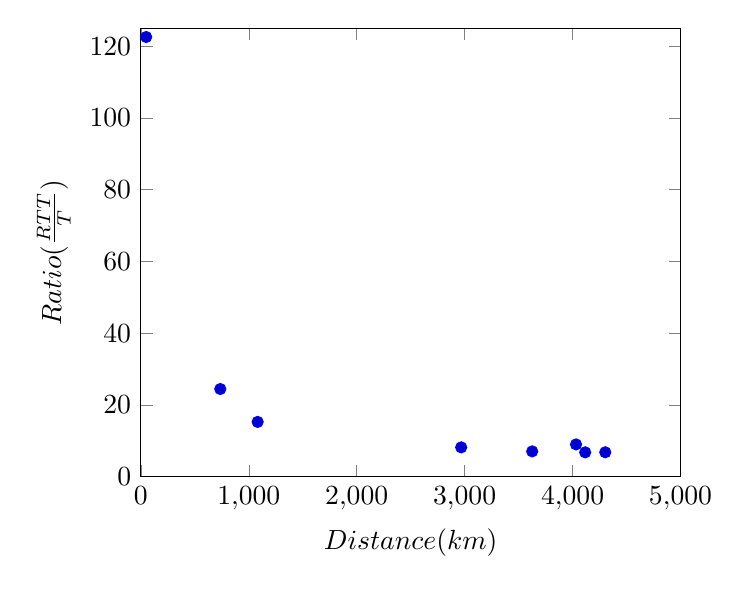
\begin{tikzpicture}
\begin{axis}[xlabel=$Distance(km)$,ylabel=$Ratio(\frac{RTT}{T})$,xmin=0,xmax=5000,ymin=0,ymax=125]
\addplot+[only marks] coordinates {
    (3626, 7.02)
    (4303, 6.77)
    (1082, 15.24)
    (736, 24.40)
    (2968, 8.14)
    (4117, 6.75)
    (4032, 8.96)
    (49, 122.55)
};
\end{axis}
\end{tikzpicture}
\item The y-values not only are all larger than 2, but they also appear to be inversely proportional to distance. The RTT to a host doesn't scale linearly with the distance to the host; it grows at a slower rate, suggesting there is some near-constant overhead in transmission when uploading bits to a network. This could be caused by relaying the packet through the 7 layers of networking at both end-hosts. There would also be delays, although probably miniscule, at each hop in the network as routers and switches process packets and their headers to forward them towards their destinations.
\end{enumerate}

\end{enumerate}

\end{document}
